% used examples from:
% http://tex.stackexchange.com/questions/212699/text-projection-onto-plane-in-3d-pgf-plots



% Plot planes, that stand for classes of some participants.
%%%%%%%%%%%%%%%%%%%%%%%%%%%%%%%%%%%%%%%%%%%%%%%%%%%%%%%%%%%%%%%%%%%%%%
% 3 coordinates and color
\newcommand{\plotPoint}[4]{
	% the point
	\addplot3[mark=*, color=#4] coordinates { (#1,#2,#3) };	
	
	% projections
	\addplot3[mark=none, dashed, color=#4] coordinates {(0,#2,#3) (#1,#2,#3)};
	\addplot3[mark=none, dashed, color=#4] coordinates {(#1,0,#3) (#1,#2,#3)};
	\addplot3[mark=none, dashed, color=#4] coordinates {(#1,#2,0) (#1,#2,#3)};
}

% Plot planes, that stand for classes of some participants.
%%%%%%%%%%%%%%%%%%%%%%%%%%%%%%%%%%%%%%%%%%%%%%%%%%%%%%%%%%%%%%%%%%%%%%
% 1) participant id; 2) color; 3) opacity.
\newcommand{\plotProfPlane}[3]{
	\addplot3[patch,patch type=rectangle, opacity=#3, color=#2]
		coordinates {(#1,0,0)(#1,5,0)(#1,5,5)(#1,0,5)};
}
% 1) participant id; 2) color; 3) opacity.
\newcommand{\plotRoomPlane}[3]{
	\addplot3[patch,patch type=rectangle, opacity=#3, color=#2]
		coordinates {(0,#1,0)(7,#1,0)(7,#1,5)(0,#1,5)};
}
% 1) participant id; 2) color; 3) opacity.
\newcommand{\plotGroupPlane}[3]{
	\addplot3[patch,patch type=rectangle, opacity=#3, color=#2]
		coordinates {(0,0,#1)(7,0,#1)(7,5,#1)(0,5,#1)};
}




\def\viewA{30}
\def\viewB{45}

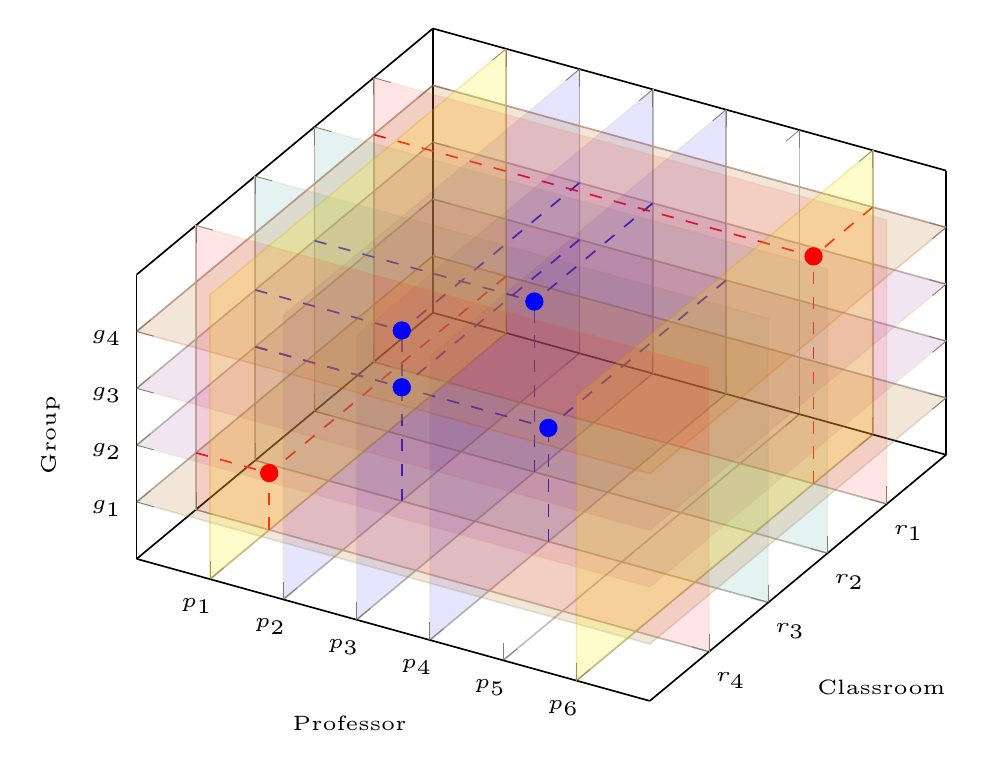
\begin{tikzpicture}[scale=1.5]
\pgfplotsset{every tick label/.append style={font=\tiny}}
\begin{axis}
[
    grid=major,
    view={\viewA}{\viewB},
% X axis
    xmin=0, xmax=7,
    	xlabel = \tiny Professor,
    xtick = {1,2,3,4,5,6},
    xticklabel=$p_{\pgfmathprintnumber{\tick}}$,
% Y axis
    ymin=0, ymax=5,
    y dir=reverse,
	ylabel = \tiny Classroom,
    ytick = {1,2,3,4},
    yticklabel=$r_{\pgfmathprintnumber{\tick}}$,	    
% Z axis
    zmin=0, zmax=5,
	zlabel = \tiny Group,
    ztick = {1,2,3,4},
    zticklabel=$g_{\pgfmathprintnumber{\tick}}$,
]

	\plotPoint{2}{3}{2}{blue};
	\plotPoint{4}{3}{2}{blue};

	\plotPoint{2}{3}{3}{blue};
	\plotPoint{3}{2}{3}{blue};

	\plotPoint{1}{4}{1}{red};
	\plotPoint{6}{1}{4}{red};

	% 2)
	\ifthenelse{ \stage = 2 }
        {
        \plotProfPlane{2}{blue}{0.1};
        \plotProfPlane{3}{blue}{0.1};
        \plotProfPlane{4}{blue}{0.1};

        \plotRoomPlane{2}{green!50!blue}{0.1};
        \plotRoomPlane{3}{green!50!blue}{0.1};
        
        \plotGroupPlane{2}{red!50!blue}{0.1};
        \plotGroupPlane{3}{red!50!blue}{0.1};
        }{}

	% 3)
	\ifthenelse{ \stage = 3 }
        {
        \plotGroupPlane{1}{brown}{0.2};
        \plotGroupPlane{4}{brown}{0.2};
        
        \plotProfPlane{1}{yellow}{0.2};
        \plotProfPlane{6}{yellow}{0.2};
        
        \plotRoomPlane{1}{red}{0.1};
        \plotRoomPlane{4}{red}{0.1};
        }{}
	

\end{axis}
\end{tikzpicture}
